\subsection{Requisitos}
Debe cumplir con una serie de requisitos técnicos mínimos para poder hacer uso de este, como son:

\begin{itemize}
	\item Conexión a internet

\item Sistema operativo:
    \begin{itemize}
        \item Windows 10/11
        \item Linux
    \end{itemize}

\item Navegador con versión minima:
    \begin{itemize}
    \item Google Chrome: 100+
    \item Mozilla: 100+
    \item Microsoft Edge: 100+
    \item Safari (macOS): 15+
    \item Opera: 85+
    \item Safari (iOS): 15+
    \item Chrome/Edge Android: Última versión
    \end{itemize}
\end{itemize}

En cuando cumpla con los requisitos anteriormente mencionados, puede continuar con el proceso de registro e inicio de sesión, de la siguiente manera:

\subsection{Acceso al sistema}

Para el acceso al sistema se cuenta con la url de acceso siguiente:

\url{ https://www.chibchaweb.site/}\\

Se encontrará en la pestaña de inicio del sitio web, donde podrá explorar los dominios, sin necesidad de registrarse.

\begin{figure}[H]
	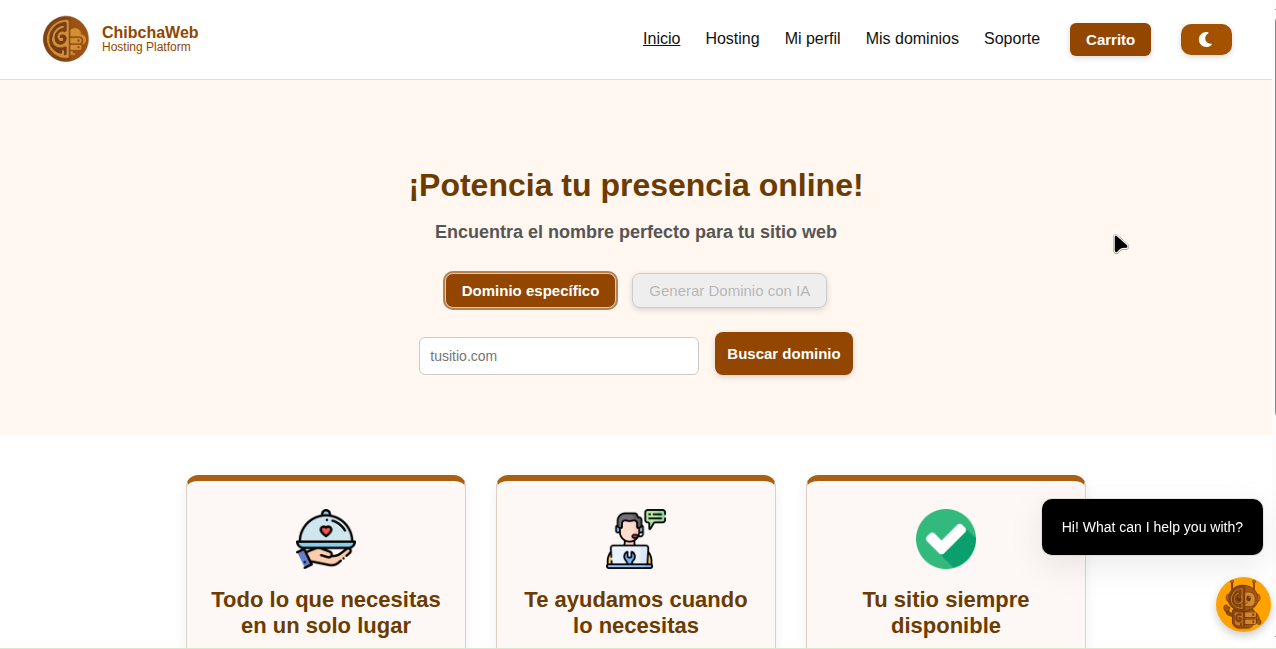
\includegraphics[width=\columnwidth]{acceso/inicio.png}
	\caption{Página principal.}
	\label{fig:inicio}
\end{figure}

\subsection{Registro de usuario }
El registro de usuario Solo se puede realizar como empleado, no como Administrador, para registrarse cómo empleado, se debe llenar el siguiente formulario:

\begin{figure}[H]
    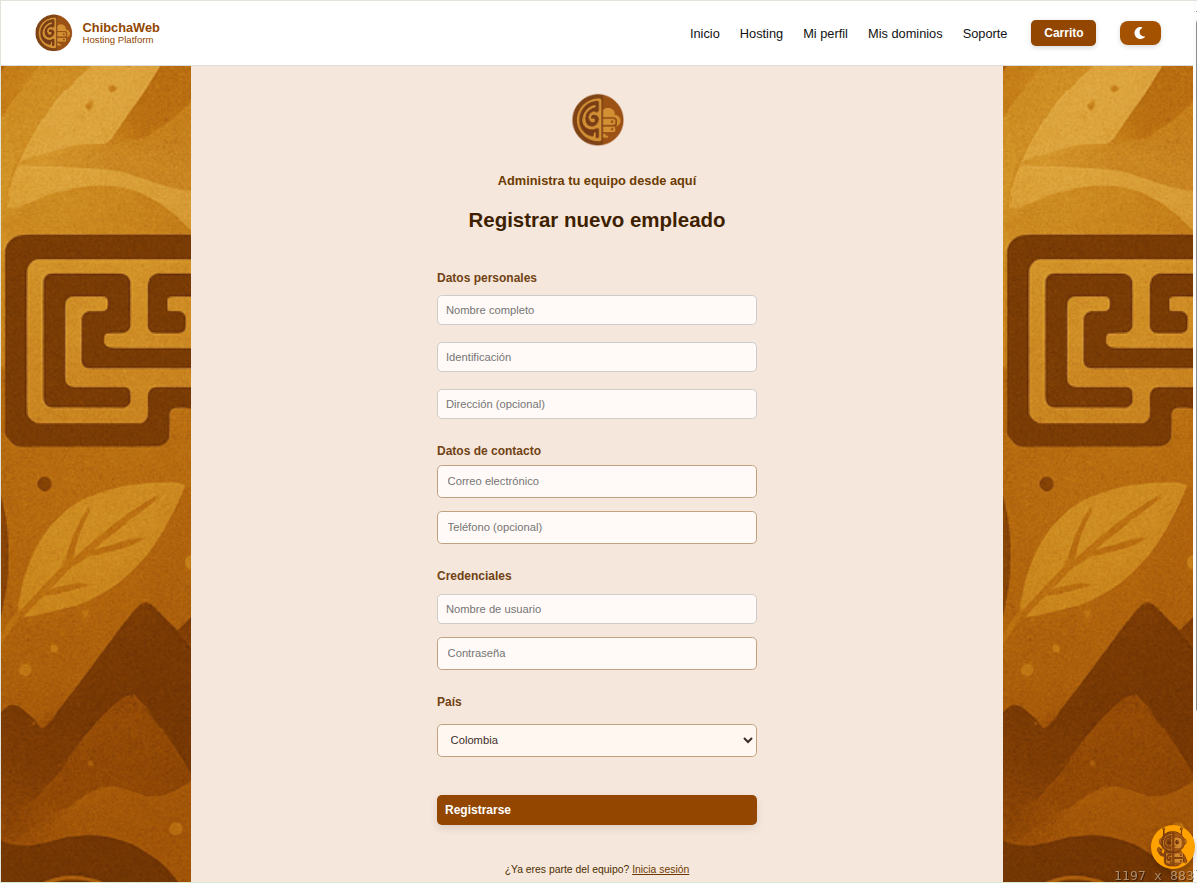
\includegraphics[width=\columnwidth]{acceso/registro-empleado.png}
    \caption{Registro empleado.}
    \label{fig:registro-empleado}
\end{figure}

Posteriormente, debe esperar a ser notificado de que su cuenta ha sido validada por un administrador.

Luego de esto será redirigido al inicio de sesión.

\subsection{Inicio de sesión}
Para el inicio de sesión, deberá ingresar su identificador de usuario, y su contraseña en los espacios que se ven en la Figura \ref{fig:login} En caso de no contar con una cuenta, revise el punto anterior.

\begin{enumerate}
	\item Dar click en el botón de “Mi perfil” que se encuentra en la barra de navegación.
	\begin{figure}[H]
		
\includegraphics[width=\columnwidth]{acceso/navbar-perfil.png}
		\caption{Barra de navegación.}
		\label{fig:navbar-perfil}
	\end{figure}
    \item Deberá ingresar sus credenciales, y dar click en “Entrar”.
    \begin{figure}[H]
        \centering
  		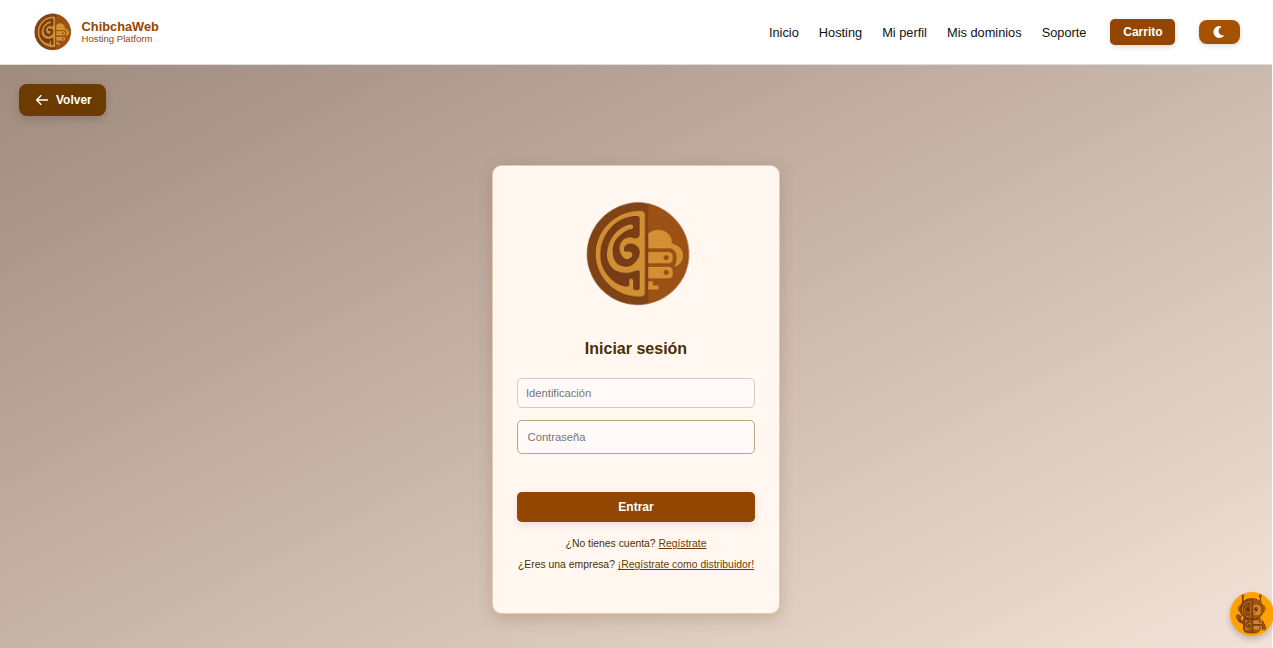
\includegraphics[width=\columnwidth]{acceso/login.png}
  		\caption{Login.}
  		\label{fig:login}
   	\end{figure}
\end{enumerate}

Luego de clic en entrar, donde deberá ver una interfaz similar a la siguiente

\begin{figure}[H]
    \centering
    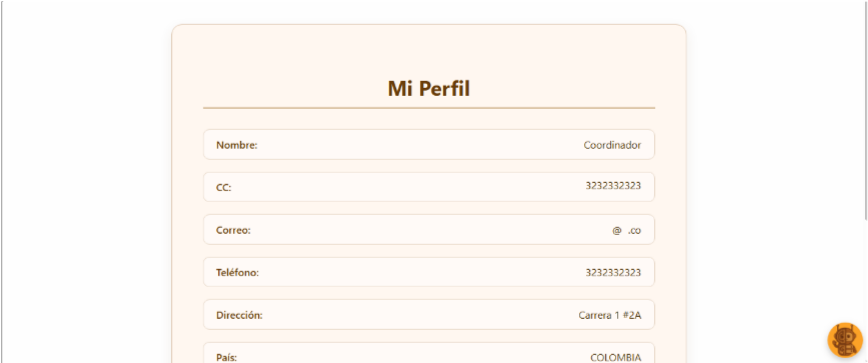
\includegraphics[width=\columnwidth]{acceso/perfil.png}
    \caption{Datos de mi perfil.}
    \label{fig:placeholder}
\end{figure}
